\section{Ekran dodawania danych}

Zdecydowano, że pierwszym ekranem aplikacji będzie ekran zapisu danych. Decyzja ta wynika z faktu, że bez przetworzonych danych, utworzenie innych ekranów byłoby zdecydowanie trudniejsze. Ekran ten składa się z elementów, które zostaną omówione poniżej.

\subsection{Zapis pliku w chmurze}
Pierwszym etapem procesu jest zapis pliku w chmurze, co umożliwia jego udostępnienie innym systemom. Do realizacji tego zadania wykorzystano kontrolkę\footnote{Kontrolka -- element służący do nawigacji, wyświetlania danych i obsługi aplikacji.} \emph{Attachment Control}. Pozwala ona na zapisanie pliku w pamięci aplikacji. Odbywa się to przez naciśnięcie przycisku \emph{"Dołącz plik"} lub przy użyciu mechaniki \emph{przeciągnij i upuść} (\english{Drag And Drop}). 

Aby przekazać plik oraz jego zawartość należy nacisnąć przycisk opisany jako \emph{Save attachments} znajdujący się pod wcześniej omawianym elementem. Naciśnięcie go skutkuje wywołaniem szeregu funkcji opisanych we właściwości \emph{OnSelect}. W pierwszej kolejności sprawdzane jest, czy plik został załadowany. Jeśli tak, to wywoływany jest przepływ \emph{SaveFileAndRunScript}. Wynik przepływu jest zapisywany w zmiennej tablicowej, która w Power Apps określana jest jako \definicja{kolekcja}, o nazwie \emph{FlowOutput}. Po wykonaniu się przepływu, pliki zapisane w pamięci aplikacji zostają usunięte.



\subsubsection{Przepływ SaveFileAndRunScript}
Rysunek \ref{fig:savefileandrunscript}, przedstawia edytor programu Power Automate. Widoczny w nim przepływ nazwany \emph{SaveFileAndRunScript} jest odpowiedzialny za zapisanie pliku w chmurze oraz wstępne przetworzenie. W momencie wywołania przepływu, plik jest przekazany jako parametr wejściowy. Przepływ ten składa się z kilku kroków, które zostaną omówione w kolejności ich wykonywania.

\begin{figure}[t]
    \centering
    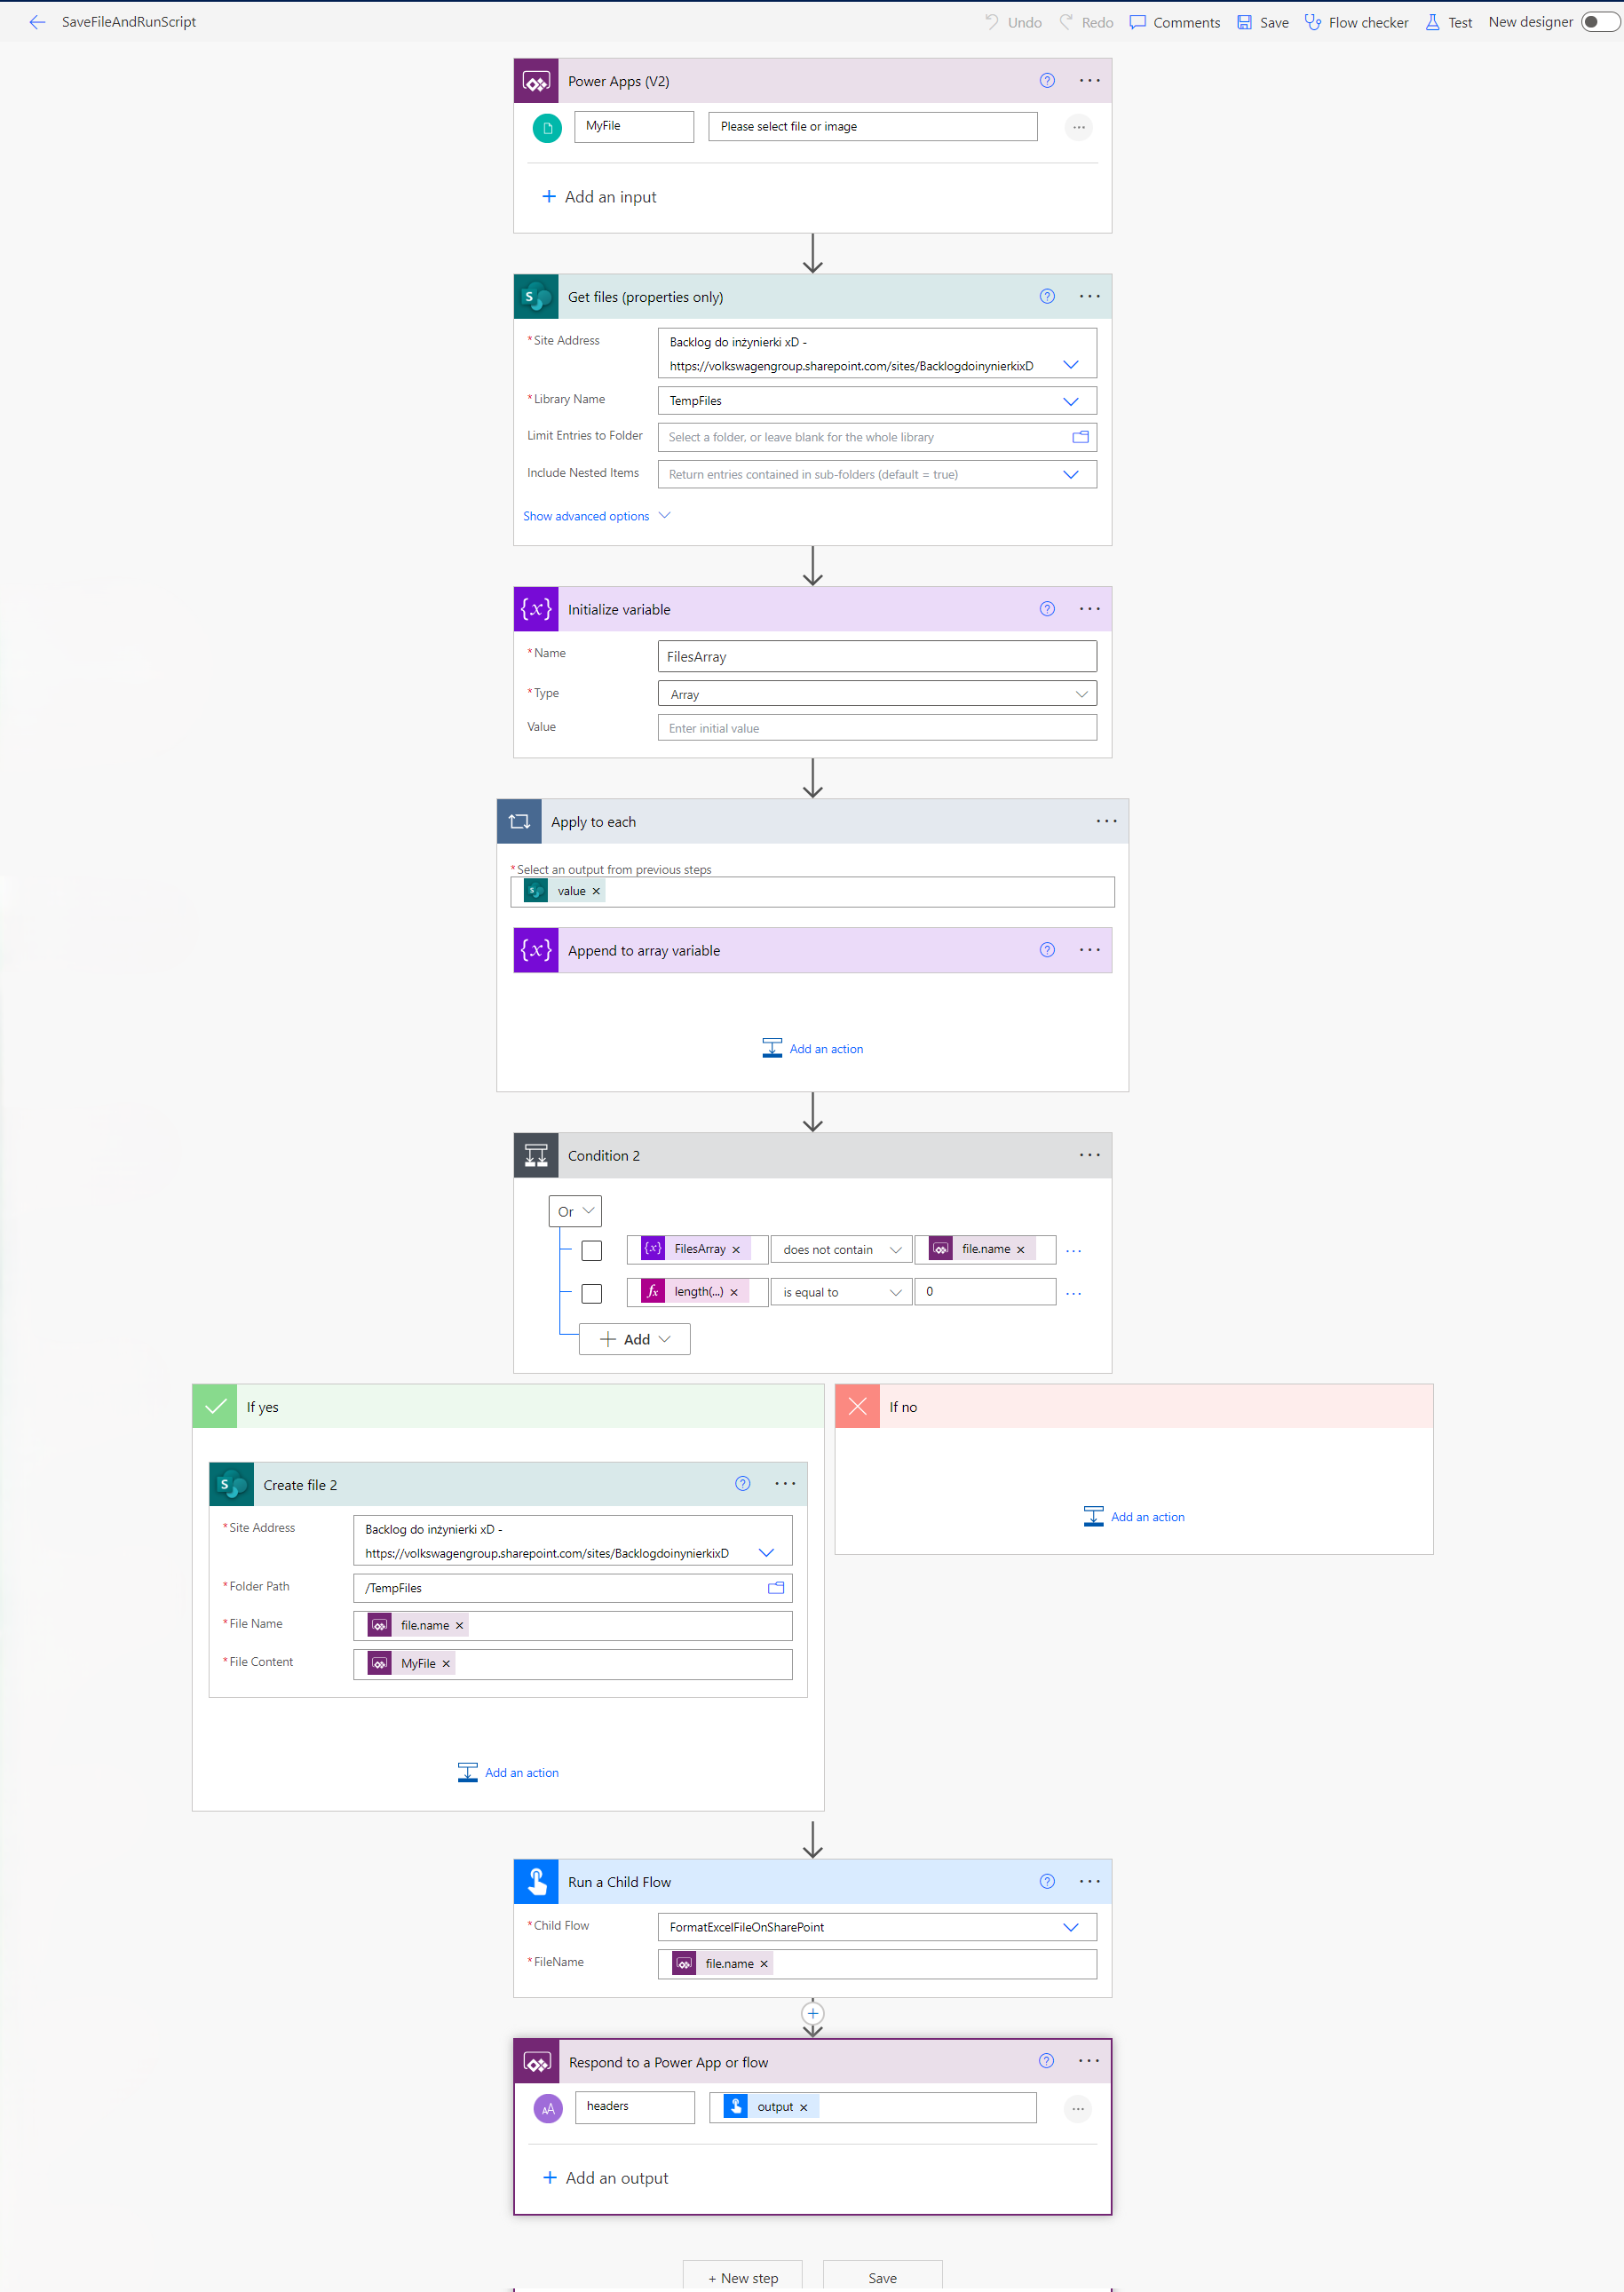
\includegraphics[width=0.9\textwidth]{figures/SaveFileAndRunScript.png}
    \caption{Widok przepływu SaveFileAndRunScript}
    \label{fig:savefileandrunscript}
\end{figure}

\begin{enumerate}
    \item \textbf{Funkcja: Power Apps (V2)} \\
    Przepływ rozpoczyna się od funkcji wywoływanej bezpośrednio z aplikacji Power Apps. Jako parametry wejściowe przyjmuje:
    \begin{itemize}
        \item nazwę pliku (\textit{File Name}),
        \item zawartość pliku (\textit{File Content}) w formacie binarnym.
    \end{itemize}

    \item \textbf{Zainicjalizowanie zmiennej} \\
    Element \textit{Initialize variable} tworzy zmienną o nazwie \textit{FileExists}, która przechowuje informację, czy plik o podanej nazwie znajduje się już na SharePoint.

    \item \textbf{Sprawdzenie istniejących plików} \\
    Blok \textit{Get files} pobiera listę wszystkich plików z wybranego folderu SharePoint wraz z ich metadanymi, takimi jak nazwa, ścieżka czy data modyfikacji. Wynik zostaje zapisany w zmiennej \textit{FileExists}, która przyjmuje wartość \textit{true}, jeśli plik został znaleziony, lub \textit{false}, jeśli plik nie istnieje.

    \item \textbf{Instrukcja warunkowa \emph{If}} \\
    Element \textit{Condition} sprawdza wartość zmiennej \textit{FileExists}. W zależności od wyniku:
    \begin{itemize}
        \item jeśli zmienna ma wartość \textit{true} -- przepływ kończy działanie,
        \item jeśli zmienna ma wartość \textit{false} -- przepływ kontynuuje proces zapisu.
    \end{itemize}

    \item \textbf{Utworzenie pliku} \\
    Blok \textit{Create file} tworzy nowy plik w SharePoint, wykorzystując parametry:
    \begin{itemize}
        \item adres witryny SharePoint,
        \item ścieżkę do folderu docelowego,
        \item nazwę pliku,
        \item zawartość pliku.
    \end{itemize}

    \item \textbf{Uruchomienie przepływu podrzędnego} \\
    Po pomyślnym zapisaniu pliku przepływ wywołuje tzw. \textit{child flow}, który inicjuje działanie skryptu Office. Skrypt ten odpowiada za przetworzenie pliku w sposób zgodny z założeniami aplikacji. Jego wynik w formacie JSON jest zwracany do przepływu nadrzędnego. 

    \item \textbf{Odpowiedź do aplikacji} \\
    Blok \textit{Respond to Power Apps} kończy przepływ, zwracając do aplikacji dane w formacie JSON, przetworzone przez wspomniany skrypt.
\end{enumerate}

\subsection{Skrypt pakietu Office}
Po utworzeniu pliku w SharePoint, w ramach przepływu następuje jego przetworzenie przez skrypt. Jego zadaniem jest dostosowanie pliku do wymagań systemu. Poniżej przedstawiono kroki działania skryptu:

\begin{enumerate}
    \item \textbf{Wybór arkusza roboczego} \\
    Skrypt identyfikuje arkusz zawierający dane, analizuje zakres używanych komórek i usuwa ochronę hasłem, jeśli jest aktywna -- krok ten jest wymagany, aby wprowadzanie zmian w arkuszu było możliwe.

    \item \textbf{Analiza danych} \\
    Skrypt rozpoczyna analizę od wyszukiwania początku tabeli w arkuszu. Następnie:
    \begin{itemize}
        \item usuwa puste kolumny, które nie zawierają żadnych danych,
        \item tworzy tabelę o dynamicznym rozmiarze, uwzględniając zakres danych znajdujących się w arkuszu,
        \item uzupełnia brakujące komórki w kluczowych kolumnach, korzystając z danych w poprzednich wierszach.
    \end{itemize}
    Takie podejście pozwala na uporządkowanie danych i przygotowanie ich do dalszego przetwarzania.

    \item \textbf{Dopasowanie nazw kolumn} \\
    Skrypt porównuje istniejące nazwy kolumn z listą standardowych nagłówków, korzystając z algorytmu \textit{Jaro-Winkler}. Algorytm ten:
    \begin{itemize}
        \item analizuje podobieństwo tekstów, porównując wspólne znaki oraz ich kolejność,
        \item przyznaje dodatkowe punkty za zgodność początkowych znaków (prefiksu),
        \item zwraca wynik jako wartość z przedziału od 0 do 1, gdzie wartości bliższe 1 oznaczają większe podobieństwo.
    \end{itemize}
    Wynik tego procesu jest wykorzystywany w dalszych etapach aplikacji, m.in. do walidacji struktury danych. Jeśli podobieństwo jest mniejsze niż 90\%, skrypt sugeruje ręczne dopasowanie nazwy kolumny.

    \item \textbf{Zwrócenie wyników} \\
    Skrypt generuje JSON zawierający mapowanie oryginalnych nazw kolumn z najlepszymi dopasowaniami z listy standardowych nagłówków.
\end{enumerate}

Wprowadzenie przepływu podrzędnego było konieczne z uwagi na sposób, w jaki Power Automate obsługuje operacje na plikach w SharePoint. Gdy plik zostaje zapisany w folderze SharePoint, system przypisuje mu status wskazujący, czy jest gotowy do przetworzenia. W przypadku realizacji obu operacji (zapisu i przetwarzania pliku) w ramach jednego przepływu pojawiał się problem. Wynikał on z faktu, że przepływ pobierał dane z SharePoint już na etapie wstępnego sprawdzenia, czy plik o określonej nazwie istnieje. Informacja ta była przechowywana w pamięci przepływu i nie była aktualizowana w trakcie jego dalszego wykonywania.

W efekcie, po utworzeniu nowego pliku, przepływ nie miał możliwości odświeżenia informacji o jego istnieniu i statusie. To powodowało błąd uniemożliwiający uruchomienie skryptu, gdyż system informował, że plik, dla którego miał być wykonany, nie istnieje.

Rozwiązaniem tego problemu było wyodrębnienie etapu przetwarzania pliku do osobnego przepływu podrzędnego. Przepływ podrzędny, uruchamiany po zakończeniu procesu zapisu pliku, działał niezależnie i pobierał aktualne dane z SharePoint w momencie swojego wywołania. Dzięki temu możliwe było wyeliminowanie problemu braku odświeżonych informacji o statusie pliku, co pozwoliło na poprawne uruchomienie skryptu Office Script.

\textcolor{red}{LINK DO TEGO JARO\_WINKLERA: https://crucialbits.com/blog/a-comprehensive-list-of-similarity-search-algorithms/}

\vspace{1cm}

\begin{figure}[H]
    \centering
    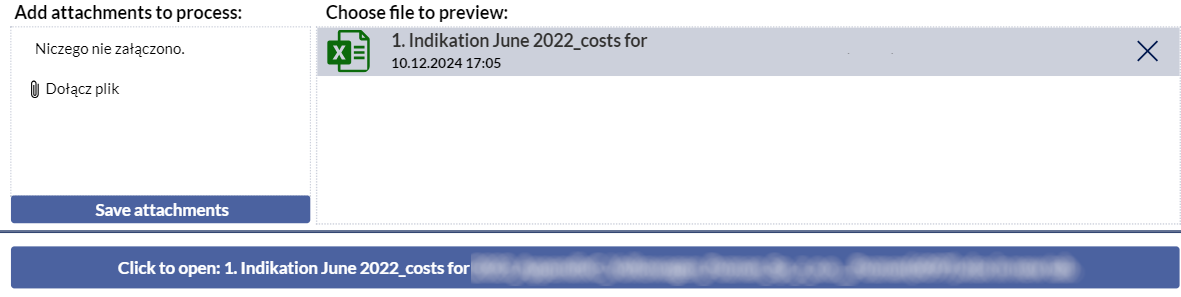
\includegraphics[width=\textwidth]
    {figures/SaveAttachmentsForm.png}
    \caption{Formularz zapisu pliku w chmurze}      
    \label{fig:saveattachmentsform}
\end{figure}

Rysunek \ref{fig:saveattachmentsform} ilustruje opisane wcześniej elementy ekranu, na którym użytkownik może dodawać załączniki do procesu, podpisane jako \emph{"Add attachments to process"}. Obok znajduje się lista zapisanych plików, umożliwiająca wybór pliku do dalszego przetwarzania. Poniżej umieszczono przycisk \emph{"Click to open:..."}, który pozwala na otwarcie wybranego pliku w nowym oknie przeglądarki, co ułatwia jego weryfikację i podgląd.

\subsection{Walidacja nazw kolumn} Kolejnym etapem przed zapisaniem danych do bazy jest walidacja nazw kolumn. W tym celu zaimplementowano formularz, którego układ przedstawiono na rysunku \ref{fig:columnmappingform}. Formularz zawiera \emph{galerię} – element umożliwiający wyświetlanie wielu rekordów danych o różnych typach. Pola wyświetlające dane w galerii mogą być dostosowywane w dowolny sposób w zależności od potrzeb użytkownika.

\noindent Galeria składa się z dwóch kolumn: \begin{itemize} \item Lewa kolumna prezentuje obecne nazwy kolumn, które są wyświetlane za pomocą kontrolki \emph{Label}\footnote{\emph{Label} -- kontrolka tekstowa umożliwiająca wyświetlanie statycznych wartości.}. \item Prawa kolumna zawiera kontrolkę \emph{ComboBox}\footnote{\emph{ComboBox} -- rozwijana lista z możliwością wprowadzania tekstu.}, umożliwiającą wybór nazwy z listy standardowych nagłówków. Lista wartości w kontrolce \emph{ComboBox} jest generowana przez skrypt opisany w poprzednich sekcjach. \end{itemize}

Po prawej stronie formularza znajduje się instrukcja użytkownika, zawierająca wskazówki dotyczące prawidłowego uzupełniania nazw kolumn. Poniżej instrukcji umieszczono przycisk \emph{Update column names}, który umożliwia wprowadzenie zmian w strukturze danych.

\noindent Działanie tego mechanizmu opiera się na zastosowaniu skryptu pakietu Office. Skrypt jako parametr wejściowy przyjmuje zmienną tablicową w formacie JSON, zawierającą mapowanie oryginalnych nazw kolumn z poprawionymi wartościami wybranymi przez użytkownika. Następnie skrypt iteruje po wierszu zawierającym nagłówki kolumn i dokonuje ich zamiany zgodnie z mapowaniem. Po zakończeniu działania skrypt zwraca nową strukturę nazw kolumn.

Rysunek \ref{fig:columnmappingform} prezentuje wszystkie elementy formularza, w tym kontrolki umożliwiające wybór roku i numeru indykacji, które zostały umieszczone pod przyciskiem \emph{Update column names}. Kontrolki te, wraz z przyciskiem \emph{Upload data}, są kluczowe dla kolejnego etapu przetwarzania danych, obejmującego ich integrację z listami SharePoint. 


\begin{figure}[t]
    \centering
    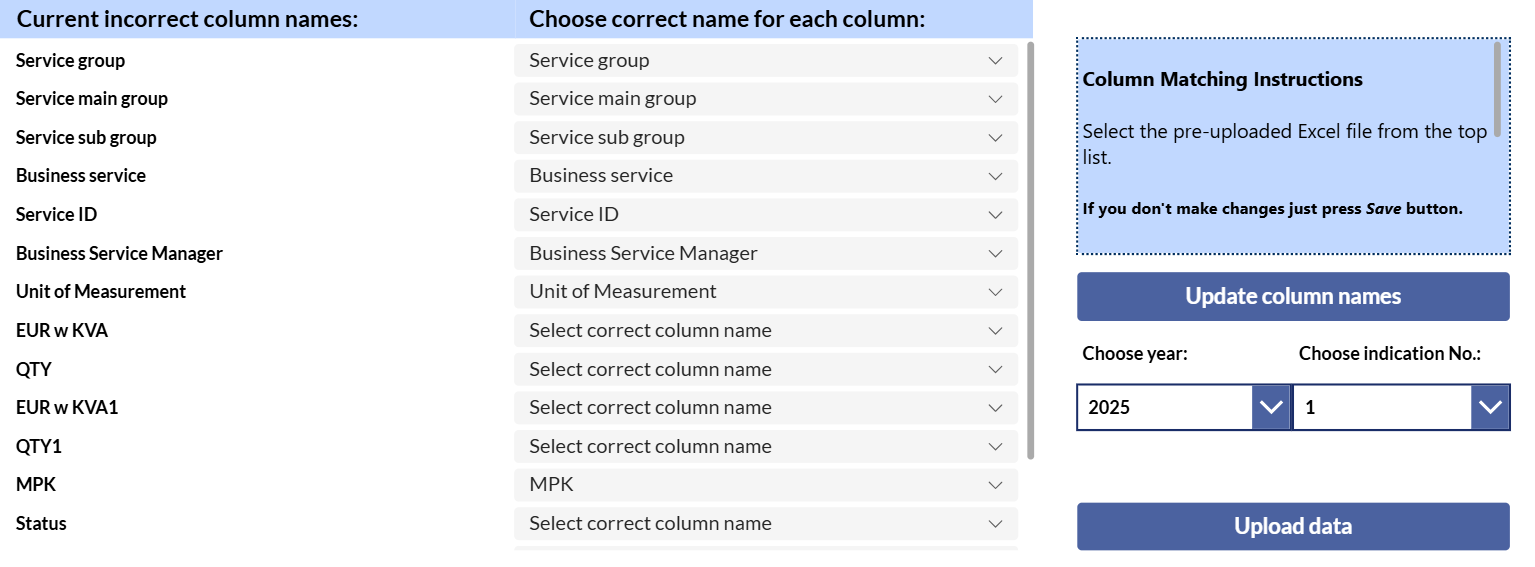
\includegraphics[width=\textwidth]{figures/ColumnMappingForm.png}
    \caption{Formularz walidacji nazw kolumn}
    \label{fig:columnmappingform}
\end{figure}

\subsection{Integracja z listami SharePoint} Po zakończeniu walidacji nazw kolumn, kolejnym etapem jest integracja przetworzonych danych z listami SharePoint. Proces ten rozpoczyna się od wyboru roku i numeru indykacji przy użyciu dedykowanych kontrolek \emph{Dropdown}\footnote{\emph{Dropdown} -- kontrolka umożliwiająca wybór jednej z dostępnych wartości z rozwijanej listy, bez możliwości edycji.}. Wybrane wartości są następnie wykorzystywane podczas importu danych do odpowiednich list, co odbywa się za pomocą przycisku \emph{Upload data}. 

Skutki kliknięcia przycisku mogą się różnić w zależności od wybranych wartości i tego czy nazwy kolumny zostały zmienione. 

\begin{figure}[htbp]
    \centering
    % Pierwszy obrazek
    \begin{minipage}{0.5\textwidth}
        \centering
        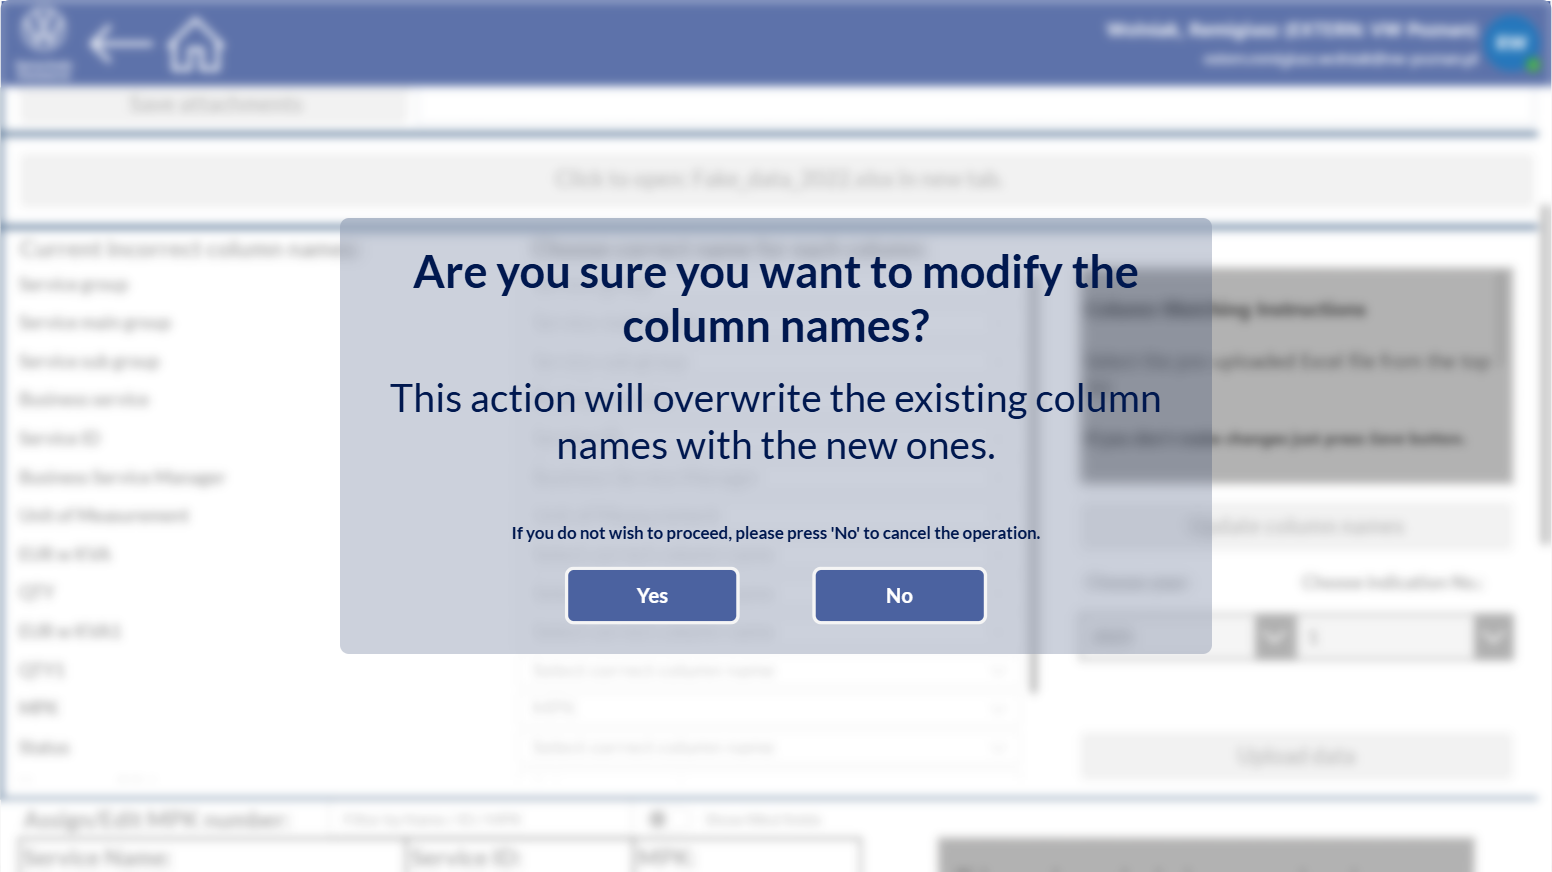
\includegraphics[width=\linewidth]{figures/CorrectHeadersPopup.png}
        \caption{Podpis pod pierwszym obrazkiem}
        \label{fig:CorrectHeadersPopup}
    \end{minipage}\hfill
    % Drugi obrazek
    \begin{minipage}{0.5\textwidth}
        \centering
        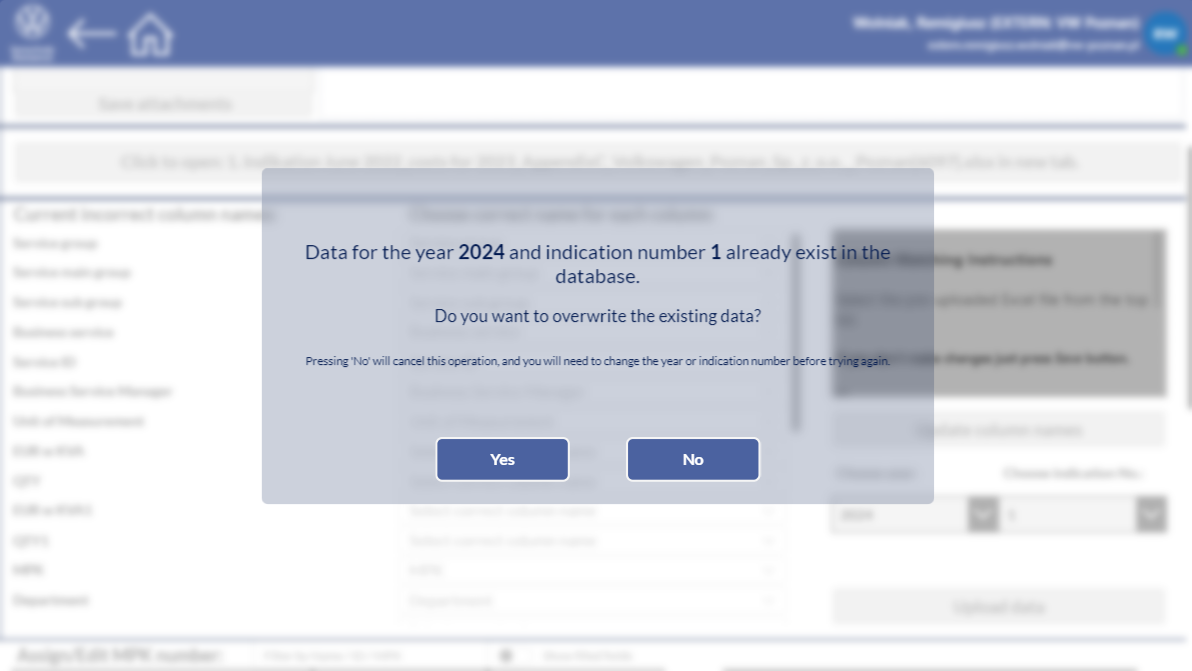
\includegraphics[width=\linewidth]{figures/DoUWantToOverwrite.png}
        \caption{Podpis pod drugim obrazkiem}
        \label{fig:DoYouWantToOverwrite}
    \end{minipage}
    \label{fig:obrazki}
\end{figure}
